%--------------------
% Packages
% -------------------
\documentclass[11pt,a4paper]{article}
\usepackage[czech]{babel}
\usepackage[utf8]{inputenc}
\usepackage{csquotes}
%\usepackage{gentium}
\usepackage{mathptmx} % Use Times Font

\usepackage[pdftex]{graphicx} % Required for including pictures
\usepackage[pdftex,linkcolor=black,pdfborder={0 0 0}]{hyperref} % Format links for pdf
\usepackage{calc} % To reset the counter in the document after title page
\usepackage{enumitem} % Includes lists

\frenchspacing % No double spacing between sentences
\linespread{1.2} % Set linespace
\usepackage[a4paper, lmargin=0.1666\paperwidth, rmargin=0.1666\paperwidth, tmargin=0.1111\paperheight, bmargin=0.1111\paperheight]{geometry} %margins
%\usepackage{parskip}

\usepackage[all]{nowidow} % Tries to remove widows
\usepackage[protrusion=true,expansion=true]{microtype} % Improves typography, load after fontpackage is selected

\usepackage{lipsum} % Used for inserting dummy 'Lorem ipsum' text into the template
\usepackage[
backend=biber,
style=iso-numeric,
]{biblatex}
\usepackage{hyperref}
\usepackage{caption}
\usepackage{subcaption}

\addbibresource{zprava.references.bib}

%-----------------------
% Set pdf information and add title, fill in the fields
%-----------------------
\hypersetup{  
pdfsubject = {},
pdftitle = {IMS - Simulační studie},
pdfauthor = {Lukáš Wagner, Radek Veverka}
}

%-----------------------
% Begin document
%-----------------------
\begin{document} 

\begin{titlepage}
   \begin{center}
       \vspace*{1cm}

       \textbf{Simulační studie k projektu IMS}

       \vspace{0.5cm}
        Téma č. 1: Epidemiologické modely pomocí celulárních automatů 
            
       \vspace{1.5cm}

       \textbf{Lukáš Wagner, Radek Veverka}

       \vfill
            
       Fakulta informačních technologií\\
       VUT v Brně\\
       prosinec 2020\\
       
   \end{center}
\end{titlepage}

\tableofcontents
\newpage

\section{Úvod}

Tato studie se zabývá zkoumáním a simulací šíření viru \emph{SARS-CoV-2}, který způsobuje onemocnění \emph{COVID-19}. 
Zkoumanou lokací je supermarket o rozloze přibližně 600$m^{2}$, který denně navštíví stovky zákazníků. 
Cílem studie je zjistit, jaký vliv budou mít určitá pravidla a omezení aplikovaná na pohyb zákazníků mezi regály v obchodě. 
Má smysl postavit zábrany mezi regály tak, aby všichni museli projít obchod připravenou cestou namísto nahodilého procházení mezi regály?  
Má smysl také nařídit minimální odstupy mezi osobami? Bude po těchto změnách z obchodu vycházet méně čerstvě infikovaných než za standardních podmínek? 
Studie se pokusí tyto otázky objasnit pomocí modelu založeném na principu celulárních automatů. 

\section{Fakta}

\subsection{Dynamika šíření virových částic}
Přenos virových částic vzduchem se skládá z hlavních tří fází: Vydechnutí kapánek, Přenos, Vdechnutí \cite{math-model}. Každá tato fáze je ovlivněna několika
proměnnými. Celý přenos je popsán nerovnicí přenosu nákazy vzduchem \ref{fig:CAT}. Jedná se o upravenou Drakeovu rovnici.
\begin{figure}[h!]
    \caption{Nerovnice přenosu nákazy vzduchem, převzato z \cite{math-model}}
    \label{fig:CAT}
    \begin{center}
      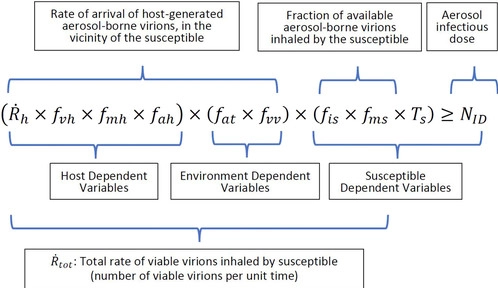
\includegraphics[width=0.8\textwidth]{spread_equation.png}
      \end{center}
\end{figure}    
Tato upravená verze předpokládá existenci prahu nákazy představující počet vdechnutých částic,
po němž se již člověk nakazí. Zbytek nerovnice popisuje, kolik částic se dostane od nakaženého člověka ke vdechujícímu člověku.

Pro výpočet tohoto množství je důležité znát počet částic na objem vzduchu vydechovaných nakaženým člověkem za jednotku času a stejně tak objem vzduchu
za jednotku času vdechnutý ohroženým člověkem. Mezi těmito dvěma stavy se virus šíří, usazuje a ukončuje aktivitu.
Šíření viru je velmi proměnná veličina závislá na proudění vzduchu. Virus opadá s rychlostí usazování mikrometrických částic z výšky
zdroje, člověka. Ukončení aktivity viru je odvozené od jeho poloviční doby života, což je v případě SARS-CoV-2 1.1h \cite{emission}.
Další důležitou proměnou je poměr výměny vzduchu ventilačním systémem. V případě mechanicky ventilovaného obchodu je tento poměr 1.1 $h^{-1}$ \cite{emission}.
Člověk nemocný Covidem-19 vydechuje přibližně 142 quanta $h^{-1}$, za předpokladu lehkého cvičení jako pohybu a tichého či žádného mluvení \cite{emission}.
Jedno quantum je množství virových částic schopných z 63\% nakazit průměrného člověka \cite{emission}.
Přesněji řečeno, quantum je definováno tak, že pravděpodobnost nákazy člověka se řídí podle exponenciálního pravděpodobnostního rozložení s parametrem $\lambda = 1$ \cite{spread-sim}

\begin{figure}[h!]
  \caption{Distribuční funkce pravděpodobnosti nakažení osoby v závislosti na vdechnutých kvantech viru, v intervalu $<0,3>$ . Vygenerováno nástrojem \href{https://wolframalpha.com}{https://wolframalpha.com}}
  \label{figtes}
  \begin{center}
    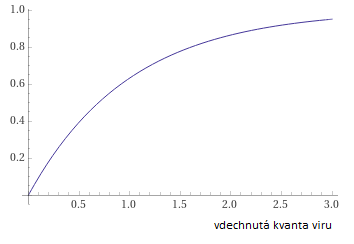
\includegraphics[width=0.8\textwidth]{exp.png}
    \end{center}
\end{figure}    

\section{Koncepty modelu a simulátoru}
\subsection{Lokace}
Místem, které má být medelováno je supermarket, zvolili jsme proto konkrétní supermarket, který známe - Tesco v Tišnově. Nákupní hala obdélníkového tvaru má rozměry zhruba 25x35$m^{2}$,
Regály jsou v prostoru rozmístěny téměř pravidelně, jak lze vidět na schématu \ref{figtes}. Vstup do obchodu a výstup z obchodu jsou vzájemně odděleny.


\begin{figure}[h!]
  \caption{Schéma rozložení regálů v Tescu Tišnov}
  \label{figtes}
  \begin{center}
    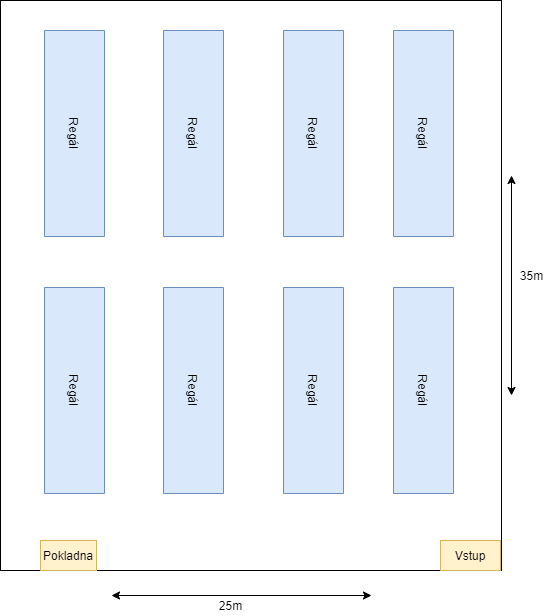
\includegraphics[width=0.8\textwidth]{tescoscheme.png}
    \end{center}
\end{figure}    

\subsection{Diskretizace prostoru pro celulární automat}
Celulární automat pracuje v poli n-rozměrného prostoru. Protože se zákaznící pohybují po zemi, což znamená že jejich vzdálenost od povrchu je konstantní, nemá příliš velký smysl simulovat jejich pohyb v trojrozměrném prostoru. Proto stav všech buňek automatu udržujeme v dvourozměrném poli.

Základní otázkou při modelování celulárního automatu je, jak velká bude jedna buňka, tedy jak velký prostor z reálného světa pokrývá. Při modelování relativně malého prostoru, jako je supermarket, je třeba vybrat velikost buňky dostatečně malou tak, aby se do celého prostoru vlezlo několik alespoň desítek buňek - simulace na 5 buňkách by nebyla přesná.
Jako hodnotu pro velikost buňky jsme zvolili \emph{0.5m} reálného prostoru. Taková velikost zajistí, že v 1 buňce se bude moci nacházet pouze jeden člověk v jednom čase.

\subsection{Diskretizace času pro celulární automat}
Simulace celulárním automatem je diskrétní, takže nepracuje souvisle v čase, ale je obnovována v pravidelných intervalech. Tento časový interval jsme zvolili \emph{1/3 s}, což znamená, že 1 sekunda reálného času je reprezentována 3 iteracemi simulátoru. Díky této hodnotě je možné simulovat chůzi člověka mezi buňkami, aniž by byly některé buňky simulátorem přeskočeny. 

\subsection{Definice stavů a okolí pro celulární automat}
Každý celulární automat má nějakou množinu stavů, ve kterých se můžou nacházet jednotlivé buňky, a tzv. \emph{okolí}, což jsou buňky, ze kterých jsou čerpána data pro přiřazení nového stavu konkrétní buňce. Stav buňky se v našem modelu skládá z:
\begin{itemize}
    \item Osoby - zdali v buňce existuje a jaké má vlastnosti.
    \item Virových částic ve vzduchu.
\end{itemize}

\subsubsection{Simulace příchodu (generování zákazníků)}
Příchod lidí do obchodu je náhodně generován v závislosti na čase. Např. v odpoledních hodinách nakupuje více lidí než v poledních. Míra příchodu lidí se řídí následovně:

\begin{center}
    \begin{tabular}{ |c|c|c|c|c|c|c|c|c|c|c|c|c|c|c|c| } 
    \hline
        hodina & 7 & 8 & 9 & 10 & 11 & 12 & 13 & 14 & 15 & 16 & 17 & 18 & 19 & 20 & 21 \\  \hline
        příchody/min & 4 & 4 & 3 & 2 & 1 & 1 & 1 & 2 & 2 & 4 & 5 & 3 & 3 & 2 & 1  \\ 
    \hline
    \end{tabular}
\end{center}

Při příchodu je každému zákazníkovi vygenerován stav popisující předchozí styk s nemocí. Stavy, jejich popis a poměr mezi zákazníky ukazuje následující tabulka:

\begin{center}
    \begin{tabular}{ |c|c|c| } 
    \hline
        stav & popis & četnost  \\  \hline
        Standardní & osoba není a nikdy nebyla nakažena & 70\%   \\ 
        Nakažlivý & osoba je aktuálně nakažena a aktivně šíří nákazu & 15\% \\
        Imunní & osoba již prodělala nákazu, nešíří ji a nemůže ji chytit & 15\% \\
    \hline
    \end{tabular}
\end{center}

\subsubsection{Simulace pohybu osob}
Základní celulární automat při výpočtu nového stavu pro buňku využívá pouze stav buňky a buňek v okolí. Při simulování pohybu zákazníků po mřížce ale v takovém případě není jak rozhodnout, kam
dál se zákazník vydá - jeho pohyb by byl nahodilý. Zákazník obvykle přijde do obchodu a zamíří k jednotlivým regálům, kde nějakou dobu stojí a vybírá zboží. Nakonec se vydá vždy na stejné místo - k pokladně. Je zřejmé, že taková simulace bude vyžadovat plánování a vyhledávání cesty. Náš simulátor simuluje pohyb osob následujícím způsobem:
\begin{enumerate}
    \item Vygeneruje se - objeví se v buňce, která značí vstup do obchodu.
    \item Naplánují se zastávky u regálů. Nahodile se vyberou buňky před regály se zbožím, kde se osoba zastaví a náhodně se vygeneruje čas zastavení.
    \item Algoritmem pro vyhledání nejkratší cesty se nalezne buňka další zastávky.
    \item Zákazník se s každou iterací posouvá buňkami blíže k zastávce.
    \item Zákazník se zastaví na zastávce na předem vygenerovanou dobu.
    \item Zastávka se vyjme z plánu, algoritmus se opakuje od bodu 3., dokud existují zastávky v plánu.
    \item Zákazník zamíří k pokladně, kde zmizí.
\end{enumerate}

\subsubsection{Simulace šíření nákazy}
Tato část simulace už opravdu využívá okolí buňky, které je nastaveno jako \emph{Mooreho okolí}. To znamená, že součástí okolí je 8 buňek, se kterými buňka sousedí. \cite{pepe-slides}
Každá buňka obsahuje parametr \emph{fumes}, což je kvantum virových částic aktuálně v buňce. Tato hodnota roste, pokud buňka obsahuje nakaženého zákazníka, který dýchá. Zároveň se část šíří do okolních buněk. Díky rozptýlení ve vzduchu a gravitaci však tato hodnota klesá s časem.

\subsection{Implementace simulátoru}
Simulátor je implementován v jazyce C++ a je přeložitelný příkazem \verb|make| na Linuxu. Každá simulace je parametrizovatelná a definovaná souborem, který obsahuje:
\begin{itemize}
    \item Seznam parametrů pro simulaci, např. doba simulace, rozložení pravděpodobnosti pro generování osob a další konstanty.
    \item Definice mapy a její velikosti. 
\end{itemize}

Pomocí argumentů programu lze konfigurovat cestu k souboru s definicí simulace, interval vypisování aktuálních statistik během simulace a interval vykreslování buňek celulárního automatu. Spuštěním bez argumentů lze zobrazit nápovědu, jak použít argumenty.

Algoritmy v simulátoru nejsou optimalizovány a vstupní data robustně ošetřována, protože toto nejsou prioritní aspekty pro studii. 

\begin{figure}[h!]
    \caption{Ukázka grafického vykreslení průběžného stavu celulárního automatu do terminálu. Černě jsou zdi a regály, bíle průchozí buňky, kružnicemi osoby. Fialovo-červené spektrum značí množství kvant viru v buňce.}
    \label{fig:render}
    \begin{center}
      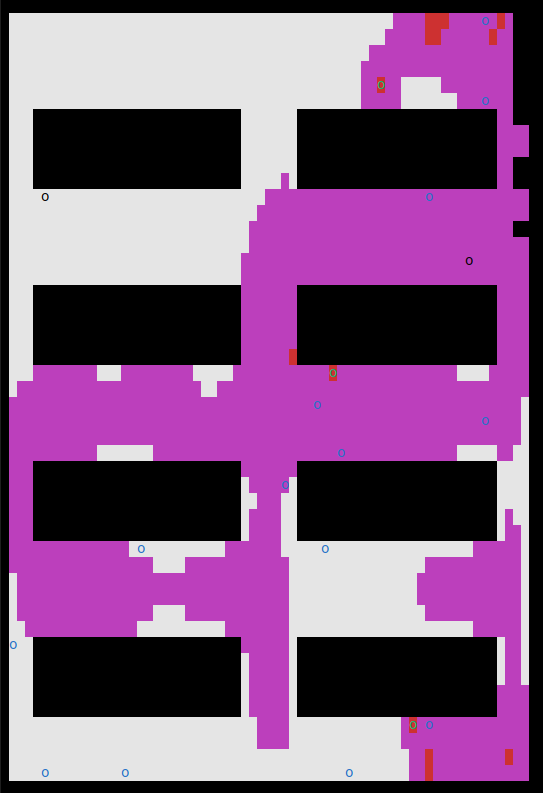
\includegraphics[width=0.6\textwidth]{graphics.png}
      \end{center}
\end{figure}    

\section{Experimenty}

\subsection{Simulace a jejich vstupy}

Základem této simulační studie jsou dvě simulace, které běží nezávisle na sobě. Obě simulace pokrývají 15 hodin reálného času, což zhruba odpovídá otevírací době supermarketů. Prostředí simulací se však liší. V první simulaci je obchod uspořádán běžným způsobem a nejsou stanovena žádná opatření pro udržování minimální vzdálenosti mezi osobami. V druhé simulaci je pohyb po obchodě výrazně omezen, jak znázorňuje obrázek \ref{twoshops}. Navíc je vynucen směr průchodu zákazníků obchodem a minimální vzdálenost, kterou musí udržovat. Ta je nastavena na 3 metry, což implikuje, že zákazníci se nemohou při průchodu obchodem předcházet (ulička není širší než 3 metry). Pokud se zákazník zastaví u regálu, musí zákazníci za ním počkat, než výběr zboží dokončí.

Téměř všechny vstupní konstanty a pravděpodobnostní rozložení jsou pro obě simulace stejné, bližší informace k nim lze najít v předchozích kapitolách této studie. Hlavními rozdíly na vstupu jsou organizace obchodu a délka dodržovaných rozestupů.

\begin{figure}[h!]
  \caption{Schéma simulovaného obchodu - vlevo pro simulaci původní, vpravo se zakázanými zónami (šedě) a přikázaným směrem nákupu.}
  \label{twoshops}
  \begin{center}
    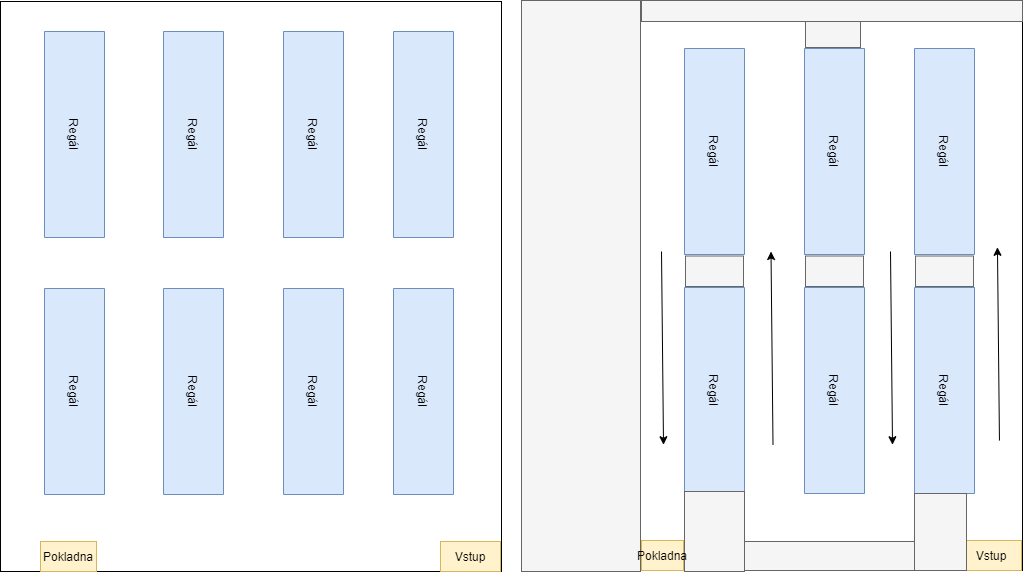
\includegraphics[width=0.9\textwidth]{tescoscheme2.png}
    \end{center}
\end{figure}    

\subsection{Výsledky simulací}
Následující tabulka udává výsledky obou simulací:

\begin{tabular}{ |c|c|c| } 
    \hline
        proměnná & simulace původní & simulace organizovaná \\  \hline
        počet zákazníků & 2296 & 1406  \\ 
        počet standardních zákazníků & 1607 & 977  \\ 
        počet nakažlivých zákazníků & 347 & 220 \\ 
        počet imunních zákazníků & 342 & 209 \\ 
        průměrná doba nákupu (minuty) & 16.9 & 11.73 \\
        průměrně vdechnuto kvant viru & 0.0401 & 0.01541 \\
        nově infikováno & 58 & 15 \\
        infekční poměr & 3.64\% & 1.566\% \\
    \hline
\end{tabular}

\section{Závěr}
Především připomeňme, že studie neřeší jak \emph{zastavit} šíření \emph{Convidu-19}, ale pouze \emph{ověřuje} jednu z možností, jak zpomalit šíření nákazy. Je třeba nakazit většinu populace, aby se vybudovala imunita, bez zásahů zpomalujících šíření by však byly přečerpány kapacity nemocnic. Druhou možností je virus kompletní izolací nechat zaniknout, toto však vyžaduje celosvětovou koordinaci a brutální zásah do ekonomiky. Studie se zaměřila na supermarkety a šíření nákazy mezi jejich zákazníky během nakupování a zkoumá případ, kdy obchod omezí pohyb zákazníků při nakupování. 

Z výsledků provedených simulací je třeba nejdříve odpovědět na otázku, jaký mají zavedená opatření vliv oproti chodu obchodu za normálních okolností.
V průběhu nakupování v rozmezí jednoho dne obchod opustilo \emph{58} nově infikovaných zákazníků, zatímco po zavedení opatření pouze \emph{15} nově infikovaných. Z toho by se dalo přinejmenším usoudit, že opatření nejsou kontraporduktivní a opravdu zpomalují šíření nákazy. Nicméně je třeba si také uvědomit, co všechno tento pokles způsobilo a jaké to má vedlejší efekty.

Důsledkem zavedení 3 metrových rozestupů je, že do obchodu se vleze mnohem méně zákazníků najednou, konkrétně cca. \emph{21} pro náš případ. 
To způsobí, že během dne obchod odbaví za normálních okolností cca. \emph{2296} zákazníku, při rozestupech však pouze \emph{1406}, což je zhruba 1.6 krát méně. Logicky, pokud obchod navštíví méně zákazníků, tak je jich i méně nově nakaženo. Abychom mohli zkoumat, zdali mají vliv i další aspekty opatření, jako je změna průchodnosti a samotné rozestupy, je třeba vyjádřít počet nakažených poměrově. Ze všech \emph{Standardních} zákazníků (těch, co nikdy nepřišli dříve do styku s nemocí), bylo bez opatření nakaženo 3.64\% a při opatření 1.566\%, což je 2,32 krát méně. Jistou roli v tomto čísle však sehraje fakt, že do obchodu přišlo méně nakažlivých lidí, pouze však zhruba 1.6 krát méně. výsledky tedy naznačují, že do sníženého počtu nově nakažených přispívají všechny faktory - menší kapacita obchodu, rozestupy a uspořádaný pohyb obchodem. 

Zkoumaná opatření je nutné dát do kontextu s dalšími opatřeními, protože studie nezahrnuje některé faktory, které by příliš komplikovaly model. Níže jsou uvedeny některé body, které je třeba si uvědomit při posuzování výsledků studie.
\begin{itemize}
    \item Nebere se v potaz usazování virových částic na zboží, pouze šíření vzduchem. 
    \item Simulace je prováděna bez roušek.
    \item U pokladen se netvoří fronty. Přepokládájí se samoobslužné pokladny (které v Tescu opravdu jsou) a schopnost lidí je rychle ovládat.
    \item Při variantě s opatřeními se tvoří fronty před obchodem. 
    \item Obchod odbaví méně lidí. Všichni si však potřebují obstarat potraviny. Bez dalších opatření a řešení by se mohlo stát, že se lidi        nahrnou do malých lokálních obchodů, kde si rozšíří virus mnohem efektivněji.
\end{itemize}

\newpage
\nocite{*}
\printbibliography[heading=bibintoc]

\end{document}
